\documentclass{template/template}

%\renewcommand{\familydefault}{\sfdefault} %% Only if the base font of the document is to be sans serif
%\usepackage{bera}

\usepackage[T1]{fontenc} % evropské uvozovky
\usepackage{subcaption}
\usepackage{amsmath}
\usepackage{enumitem}
\usepackage{hyperref}
\usepackage{gensymb} % balíček symbolů
\usepackage{booktabs}
%\usepackage{lmodern}
\usepackage{csquotes} % text lze uvést do uvozovek pomocí \enquote{text}
\usepackage{textcomp}

\usepackage[toc,page]{appendix}
\usepackage{color} % balíček pro obarvování textů
\usepackage{xcolor}  % zapne možnost používání barev, mj. pro \definecolor
\definecolor{mygreen}{RGB}{0,153,153} % nastavení barev odkazů 
\definecolor{myblue}{RGB}{0,0,200} 
\definecolor{commentgreen}{RGB}{0,100,0} % nastavení barev pro příklady z C++
\definecolor{deepblue}{rgb}{0,0,0.7}
\definecolor{deepred}{rgb}{0.6,0,0}
\definecolor{deepgreen}{rgb}{0,0.5,0}
\usepackage{listings} % balíček pro formátování zdrojových kódů 
\usepackage[author=,status=draft]{fixme} % vkládání poznámek  
% dva módy (status): draft (poznámky se zobrazují v PDF) / final (poznámky se nezobrazují v PDF)
\usepackage{graphicx}
\usepackage{multirow}
\usepackage{float}


\usepackage[T1]{fontenc} % import tučného písma typu tt pro prostředí listings
%\usepackage{listings} % balíček pro obarvování syntaxe ukázek programů v textu
\usepackage{listingsutf8} %nutné pro \usepackage{listings} aby to jelo v UTF-8
\lstset{
	extendedchars 	= false,
	language      	= C++,
	basicstyle      = \ttfamily,
	keywordstyle     = \bfseries,
	%identifierstyle = \color{brown},
	commentstyle    = \color{commentgreen},
	otherkeywords	= {self},             % Add keywords here
	emphstyle		= \color{deepred},    % Custom highlighting style
	stringstyle	 	= \color{deepgreen},		
	keywordstyle	=\color{deepblue},
	stringstyle     = \color{magenta},
} % písmo a  barvičky  by možná chtěly doladit - nějaký dobrovolník? 
% volba literate= pro znaky s diakritikou z kódů se zvýrazněnou syntaxí se nesmí používat, rozbíjí překlad

% \begin{lstlisting} Tady je zdrojový kód např. v C++ \end{lstlisting} - pro UTF-8 NE
%\lstinputlisting{source_filename.py} vloží soubor z daného místa a obarví

\usepackage{hyperref} % balíček pro hypertextové odkazy
% \url{www.odkaz.cz}
% \href{http://www.odkaz.cz}{Text který bude jako odkaz}
%\hyperlink{label}{proklikávací_text} - odkaz na text 
% \hypertarget{label}{cíl_odkazu} - cíl odkazu  


\hypersetup{colorlinks=true, linkcolor=myblue, urlcolor=mygreen, citecolor=blue, anchorcolor = magenta,
	linktocpage = true, frenchlinks } % nastavení barvy odkazů 
% bookmarksopen=true, bookmarksnumbered=true, bookmarksopenlevel=1 - nastavuje rozbalování levého menu       





%\usepackage{expl3} % bibtex dependency, must be loaded prior to the bibtex
%\usepackage[backend=bibtex,bibstyle=numeric,sorting=none,date=long,dateabbrev=false,texencoding=utf8,bibencoding=utf8,style=iso-numeric]{biblatex}

\usepackage[a4paper]{geometry}

%\lstset { 
%    language=C++,
%    backgroundcolor=\color{black!5}, % set backgroundcolor
%    basicstyle=\footnotesize,% basic font setting
%}

%\addbibresource{text.bib}
%\nocite{*}

\titlecz{Párty světla} % Název práce
\author{Anna Králová} % Jméno autora
\institution{STŘEDNÍ PRŮMYSLOVÁ A~VYŠŠÍ ODBORNÁ ŠKOLA BRNO, Sokolská 1} % Celý název instituce
\institutiontype{příspěvková organizace} % Typ instituce
\thesistype{maturitní práce}  % Typ práce/dokumentu
\mentor{Mgr. Miroslav Burda} % Jméno vedoucího práce
%\mentorstatement{Ing. Václava Zavadila} % Jméno vedoucího práce ve čtvrtém pádě

% Newly added
\authorname{Anna}
\authorsurname{Králová}
\schoolyear{2021/2022}
\field{Technické Lyceum} % Studijní obor
\class{L4A}

\placefooter{Brno 2021}

% \usepackage{hyperref} % balíček pro hypertextové odkazy
% \url{www.odkaz.cz}
% \href{http://www.odkaz.cz}{Text který bude jako odkaz}
% \hyperlink{label}{proklikávací_text} - odkaz na text 
% \hypertarget{label}{cíl_odkazu} - cíl odkazu 

%%% Přepínač pracovní kopie
%\workcopytrue
\workcopyfalse

%\renewcommand\bibname{Literatura a zdroje}

\begin{document}
\hyphenation{SOLIDWORKS Solid/-Works}

\newgeometry{margin=2cm, top=3cm, bottom=2.5cm, left=2.5cm, includefoot}

\maketitle

\newgeometry{margin=2cm, top=2.5cm, bottom=2.5cm, left=2.5cm, right=2cm, includefoot}

\makecopyrightstatement{V~Brně}



\pagestyle{empty}

\section*{Zadání}

Cílem této ročníkové práce je sestrojit fukční prototyp světel za použití programovatelného, inteligentního LED Pásku. 


%\subsection*

\vspace{20mm}

%\section*

%\subsection*

\newpage
\pagestyle{plain}

\tableofcontents % vysází obsah

\setlength{\parskip}{0.4em}

%%% Začátek práce
\setcounter{figure}{0}
\setcounter{table}{0}
\newpage

% Úvod práce
\chapter*{Úvod}
\addcontentsline{toc}{chapter}{Úvod}

 %(viz kapitola \ref{3_kap}).
Každý z nás má rád malé dekorace. Ať už jsou to malé sošky, které pokládáme na poličky v našich pokojích, nebo obrovské vázy, či kusy drúz na ozdobení našich obývacích pokojů. Dekorace ale nemusí být jen takto jednoduchá. Občas se může jednat i o lampičky roztodivných tvarů, nebo vodní mlýnky, které v sobě mají zabudované LED a pomocí cirkulující vody se paprsky světla lámou dopadají na stěnu, což by se dalo nazvat dekorací samo o sobě.
%\cite{schommers}

Mě osobně se vždycky líbily malé průhledné stromečky, které se prodávaly na Vánoce a~jejich barva se postupně měnila. A tak mě napadlo, proč něco takového také nevyrobit, ale tentokrát místo stromečku použít tvar nějaké květiny, která by měnila barvu světla podle ovládání. %(viz kapitola \ref{3_kap}).


Cílem této ročníkové práce je sestrojit prototyp takového dekoračního světla, včetně naprogramování inteligentního LED pásku, dokumentace a možných návrhů, jak tento nápad inovovat.
%\href{https://www.tecomat.cz/products/}{teco}

%todo zadání

%todo odkaz na knihovny

%todo (viz kapitola \ref{3}) --> otázka na učitele?


%Vložíme podle návodu autora programu
%moduluje wifina
%V módech světla -- reference na poslední kapitolu
%Vytvořit na Githubu sloéžku pro původní program, který jsem poté upravila
%přidat subchapters do 4. a 5. kapitoly
%Pájení --> obrázek zapájené soustavy DevKitC a LED 
%Rozepsání se, co je Visual Studio Code Zač
%Propagace letního robotického tábora

%Odkazy? Github?


\chapter{Elektronika}

\section{Součástky}
V této kapitole jsou shrnuty a~popsány veškeré elektronické součástky, které jsem v~realizování maturitní práce použila.
Na obrázku 1.1 je schematické zapojení použitých součástek.

\begin{figure}[htbp]
	\centering
	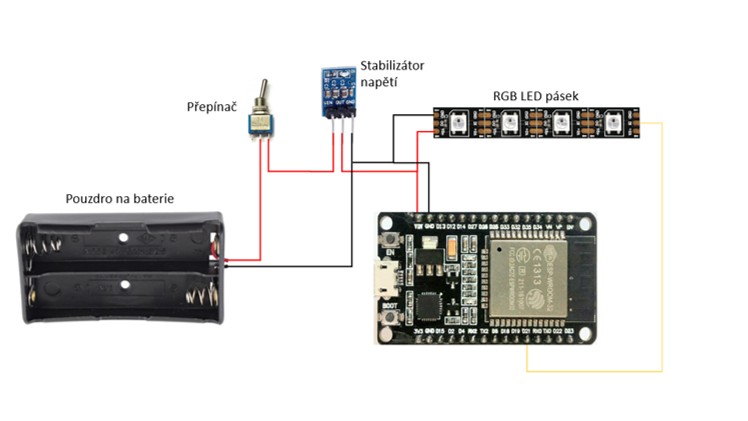
\includegraphics[width=1\textwidth]{img/01 uvod/RGB Schema.png}
	\caption{Blokové schéma obvodu}
	%	\label{fig:install-sdk-3}
\end{figure}

\subsection{ESP32-DevkitC}
\textit{ESP32-DevKitC}\cite{devkitc-datasheet} je výkonný programovatelný mikročip s WiFi a Bluetooth modulem, vyvinutý společností Espressif\cite{espressif}. Je kompatibilní s Arduinem\cite{arduino}, se kterým se často využívá v~domácích hobby projektech. WiFi a Bluetooth modul dovoluje uživateli se na \textit{ESP32-DevKitC} připojit pomocí jakéhokoliv dálkového ovladače, nebo mobilního telefonu a se zařízením manipulovat.
Součástí \textit{ESP32-DevKitC} desky je také micro-USB konektor, který dovoluje jak jednoduché nahrávání programu, tak jednoduché napájení. Pro další manipulaci a využití se~po obou stranách desky nachází vstupní a výstupní programovatelné piny, díky kterým lze k \textit{ESP32-DevKitC} připojit periferní zařízení, nebo zdroj napájení.

\begin{figure}[htbp]
	\centering
	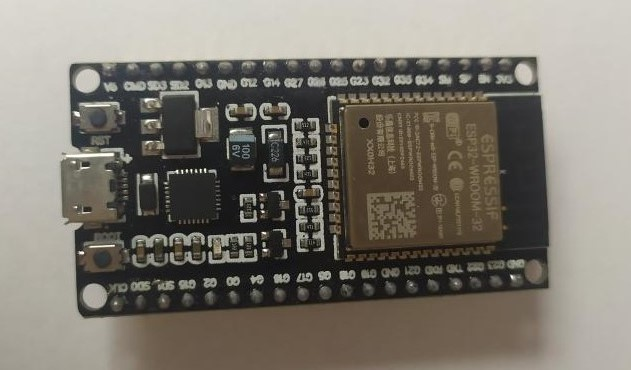
\includegraphics[width=0.5\textwidth]{img/02 ele/ESPDevKit3.jpg}
	\caption{\textit{ESP32-DevKitC v4}}
	%	\label{fig:install-sdk-3}
\end{figure}

Při realizaci maturitní práce byly použity dvě verze desek: novější verze \textit{ESP32-DevKitC v4} a stejně výkonnou, ale vývojově o malinko starší verze \textit{ESP32-DevKitC v1}. Rozměry obou desek jsou 55~mm x 30~mm a liší se pouze pozicí a označením vstupních a výstupních pinů. Jinak je práce a manipulace s nimi stejná. 

\subsection{LED pásek WS2812}

Jedná se o programovatelný ohebný LED pásek, který se z důvodu nízké spotřeby a estetického vzhledu často využívá jako páskové osvětlení do interiérů a exteriérů. Pásek se~skládá z řady LED typu \textit{WS2812}\cite{WS2812}, které se pomocí kontroléru ve WS diodách dají jednoduše programovat. 

\begin{figure}[htbp]
	\centering
	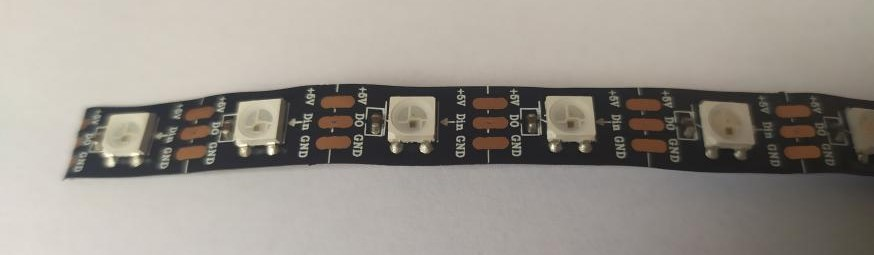
\includegraphics[width=0.5\textwidth]{img/02 ele/OhebnyLedPasek2.jpg}
	%<<<<<<< Updated upstream
	\caption{Pásek WS2812}
	%=======
	%	\caption{Pásek ws2812}
	%>>>>>>> Stashed changes
	%	\label{fig:install-sdk-3}
\end{figure}

Tento pásek se také často využívá jako výstupní modul pro \textit{Arduino}. Lze ho sehnat v~každém obchodě s elektronikou a elektrotechnickými součástkami, často pod marketingovým označením Neopixel\cite{neopixel}. 

\subsection{DC Regulátor napětí 5,5V}

% DollaTek 5,5V DC Voltage Regulator Step Down
Regulátor v obvodu slouží pro sražení vysokého napětí na napětí požadované. Tento DC~Regulátor napětí\cite{DollaTek} sráží 5,8~V až 12~V na napětí 5~V. Sama deska \textit{ESP32-DevKitC} obsahuje vlastní stabilizátor, který sráží napětí z 5~V na 3,3~V. Jmenovité napětí LED pásku je 5~V. Pokud by tedy bylo do obvodu puštěno vyšší napětí, mohlo by dojít jak ke zničení LED pásku, tak desky \textit{ESP32-DevKitC}.



    \begin{figure}[htbp]
	\centering
	\begin{minipage}[b]{0.5\textwidth}
		\centering
		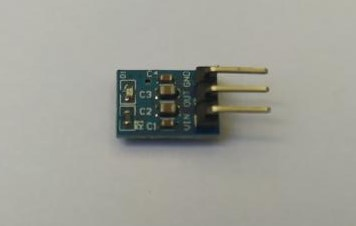
\includegraphics[width=0.75\textwidth]{img/02 ele/Stepdown front.jpg}
		\caption{Stabilizátor zepředu}
		%		\label{fig:gear-sketch1}
	\end{minipage}
	\qquad
	\begin{minipage}[b]{0.4\textwidth}
		\centering
		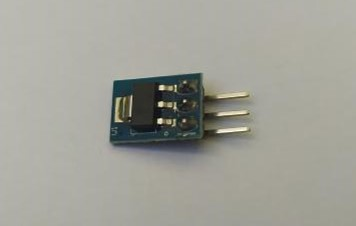
\includegraphics[width=1\textwidth]{img/02 ele/Stepdown back.jpg}
		\caption{Stabilizátor zezadu}
		%		\label{fig:gear-sketch2}
	\end{minipage}
\end{figure}


\section{Možnosti Napájení}

Důležitou součástí obvodu je také napájení, které by mělo mít dostatečně vysoké napětí, aby mohlo napájet obvod. Napájecí napětí obvodu muselo být minimálně 5~V. Napadly mě 3 možnosti řešení napájení ESP32-DevKitC a LED pásku.


\subsection{4x AAA baterie 4.8V}

Prvním nápadem bylo využít 4 tužkové AAA baterie s napájecím napětím 1,2~V, zapojené do série tak, aby jejich výsledné napětí byla 4,8~V. Tato možnost se jevila velmi výhodně, protože vzhledem k nízkému napětí nebyl potřeba v obvodu regulátor napětí, a sehnat AAA tužkové baterie je velmi jednoduché. Nevýhodou ale bylo, že by držák na 4 AAA tužkové baterie zabíral v základně hodně místa.
\newpage
Později se ale ukázalo, že není možné využít této možnosti, protože jmenovité napětí LED pásku bylo přesně 5,0~V, a i přesto, že ESP32-DevKitC fungoval bezchybně i na 4,8~V, LED pásek neměl dostatečně vysoké napětí, aby fungoval. Proto bylo potřeba zvážit jinou alternativu.


\subsection{Napájení Powerbankou}

Další možností bylo využít konektoru, který byl součástí desky  ESP32-DevKitC a přes něj napájet Powerbankou.

Výhoda tohoto napájení je, že v obvodu by nebyl potřeba stabilizátor. ESP32-DevKitC je schopno si samo, pomocí svého regulátoru, srážet převyšující napětí a napájet LED pásek pouze na 5V. Při realizaci této možnosti by nebylo potřeba řešit ani baterie, ani regulátor a celkově by se tato možnost vyplatila jako rychlé řešení problému. 

Co se týče umístění powerbanky. Byly zde opět dvě možnosti: %Nenapadlo mě jak jinak to formulovat
První možnost byla sehnat dostatečně malou powerbanku, aby se dala zabudovat do základny společně se zbytkem obvodu. 
%todo Je vážně správné slovo externí? 

Další možností bylo používat powerbanku jako externí zdroj, kdykoliv by bylo potřeba světla napájet. Oproti minulé možnosti by mohla mít powerbanka jakoukoliv velikost a tvar a~kdyby bylo potřeba, mohla by být nahrazena napájením z počítače nebo jakýkoliv kabelem.  

Stejně tak by nebyl problém s opakovatelným nabíjením Powerbanky.  V případě, že by Powerbanka byla zabudovaná vevnitř, stačilo by ji vytáhnout a znovu přes USB kabel nabít. 
V případě, že by Powerbanka sloužila jako externí zdroj, bylo by její znovunabíjení ještě jednodušší.
%(kdyby se powerbanka zabudovala dovnitř, základna by byla o mnoho větší než výsledná žárovka a kazilo by to estetický dojem, Dále jsem chtěla, aby byla světla autonomní, aby stačilo pouze zapnout tlačítko. Nelíbila se mi představa, že ze světla bude vést kabel až k powerbance.)


\subsection{Li-ion 18650}

Jako nejvhodnější možnost se mi ale jevilo využití dvou sériově zapojených Li-ion baterií 18650\cite{liion} o napětí 3,6~V (dohromady 7,2~V), jejichž napětí by se muselo srazit regulátorem napětí, ale zajišťovaly dostatečné napětí jak pro ESP tak pro LED. Rozměry baterií v držáku byly 75~mm x 42~mm x 20~mm.  Takže baterie byly dostatečně malé, aby se mohly uložit do základny se zbytkem obvodu. Li-ion baterie lze opakovaně nabíjet na speciální akumulátorové nabíječce, čímž se po delší době může výstupní napětí baterií malinko snížit, což ale v našem případě nevadí, protože přebytek napětí na bateriích je dostatečně vysoký, abychom se nemuseli bát nedostačujícího napětí. 


\begin{figure}[htbp]
	\centering
	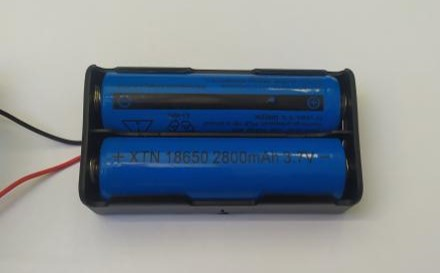
\includegraphics[width=0.45\textwidth]{img/02 ele/Battery_Pack.jpg}
	\caption{Baterie}
	%	\label{fig:install-sdk-3}
\end{figure}



%Chtěla jsem aby zařízení bylo autonomní


\section{Nabíjení}
Nabíjení by v případě použití čtyř tužkových baterií AAA, nebylo potřeba vůbec řešit, protože pokud by se baterie vybily, stačilo by jednoduše koupit nové. Stejně tak by nebyl moc velký problém při použití powerbanky, protože v případě vybití by stačilo powerbanku jednoduše znovu nabít.

S nabíjením Li-ion baterií to je ale trochu složitější. Ne každý doma vlastní speciální akumulátorovou nabíječku na Li-ion baterie, takže vyřešení nabíjení baterií je oproti dvěma předchozím možnostem napájení o malinko složitější. 
% Tato nabíječka ale není běžnou součástí každé domácnosti. 
Pro vyřešení této problematiky byla použita součástku \textit{TP4056}\cite{TP4056}.


\subsection{Nabíječka Li-ion článku TP4056 micro-USB}
Jedná se o nabíjecí čip, určený pro nabíjení lithiových akumulátorů, který při připojení k~držáku na baterie dovoluje pomocí micro-USB konektoru dané baterie nabíjet. Modul nemá zkratovou ochranu, proto je při práci s ním potřeba opatrnost. Ochrana proti přepětí modulu je do 4,2V, takže pro nás ideální. Dále jsou součástí modulu dvě indikační LED. Červená LED indikuje nabíjení. Modrá LED indikuje kompletní nabití. 

\begin{figure}[htbp]
	\centering
	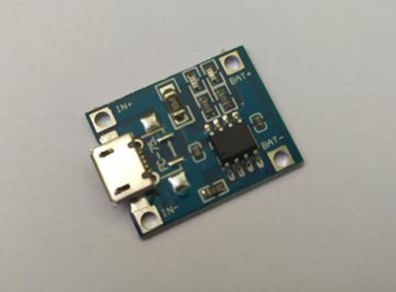
\includegraphics[width=0.3\textwidth]{img/02 ele/Napajeci clanek.jpg}
	\caption{Nabíjecí článek}
	%	\label{fig:install-sdk-3}
\end{figure}

Nabíjení pomocí tohoto článku se dá opět vyřešit dvěma způsoby.

\begin{enumerate}
	\item Připojit nabíjecí modul přímo do obvodu
	\item Vytvořit vlastní nabíječku
\end{enumerate}


\subsection{Připojit modul do obvodu}
Jedna ze dvou možností bylo připojit nabíjecí článek přímo do obvodu k bateriím, aby v~případě jejich vybití stačilo sundat vrchní díl základny a pomocí micro-USB konektoru na~modulu obě baterie znovu nabít.
Takhle metoda se mi zdála nevhodná z důvodu, že by základna po celou dobu nabíjení baterie musela být otevřena. 


\subsection{Vlastní nabíječka}
%Vytvořit pomocí nabíjecího článku a držáku na baterky vlastní nabíječku
Druhá možnost se mi jevila podstatně přijatelnější. Plánem bylo vzít držák pro dvě baterie a na jeho vývody napájet 2 nabíjecí články. Na každou jednotlivou baterii se napájel článek zvlášť, protože článek neumí napájet baterie v sériovém zapojení.

Tato možnost se jevila jako vhodná a levná alternativa, jak vyřešit nabíjení baterií. 
%Problémem zůstává, že vyndávání Li-ion baterií, aby mohli být umístěny do nabíječky, bude celkem obtížné. V tu chvíli se ale tato možnost jevila mnohem jednodušeji, než znovu předělávat celý obvod.
%Bohužel jsem se spletla a zapájela to obráceně. No… Asi to nebylo tak jednoduché jak jsem psala. 

    \begin{figure}[htbp]
	\centering
	\begin{minipage}[b]{0.45\textwidth}
		\centering
		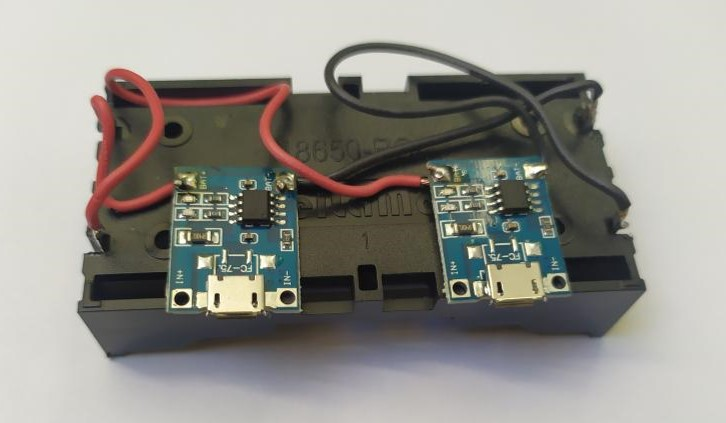
\includegraphics[width=1\textwidth]{img/02 ele/Nabijecka.jpg}
		\caption{Nabíječka zepředu}
		%		\label{fig:gear-sketch1}
	\end{minipage}
	\qquad
	\begin{minipage}[b]{0.45\textwidth}
		\centering
		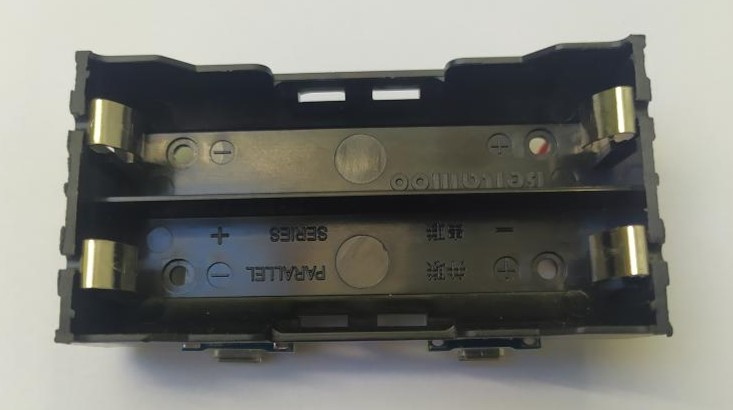
\includegraphics[width=1\textwidth]{img/02 ele/Nabijecka 2.jpg}
		\caption{Nabíječka zezadu}
		%		\label{fig:gear-sketch2}
	\end{minipage}
\end{figure}
\newpage





\chapter{Ovládání}
Ovládání LED světel bylo zajištěno pomocí WiFi modulu, jenž součástí ESP32-DevKitC. Plánem bylo připojit mobilní telefon na WiFi modul a využít ho jako dálkový ovladač. 

Toho bylo dosáhnuto za pomoci aplikace RBController, což je aplikace speciálně Robotárnou navržena na řízení a ovládání desek za pomoci WiFi Modulu. Na Robotárně už se spoustu let využívá pro dálkové řízení robotů pomocí mobilních telefonů. Tato aplikace byla také použita na Letním Robotickém táboře 2020, který každoročně pořádá Helceletka.

Prvním krokem bylo si ale v aplikaci vytvořit a umístit tlačítka na řídící plochu tam, kde jsem je chtěla mít. A přesně k tomu jsem využila webovou aplikaci Esp32-RBGridUI-Designer, speciálně Robotárnou navrženou pro tuto práci


\section{\href{https://roboticsbrno.github.io/Esp32-RBGridUI-Designer/}{Esp32-RBGridUI-Designer}} 
Esp32-RBGridUI-Designer je webová aplikace, vytvořena Robotárnou za účelem navrhnutí ovládacího panelu, který se zobrazí v aplikaci RBController, při připojení uživatele k WiFi modulu. 

Webová aplikace dovoluje uživateli určit počet, barvu a umístění tlačítek na ovládacím panelu. Aplikace má příjemné prostředí a dobře se s ní pracuje. 

Webová stránka {\em Esp32-RBGridUI-Designer} má toto rozložení: 


\begin{figure}[htbp]
	\centering
	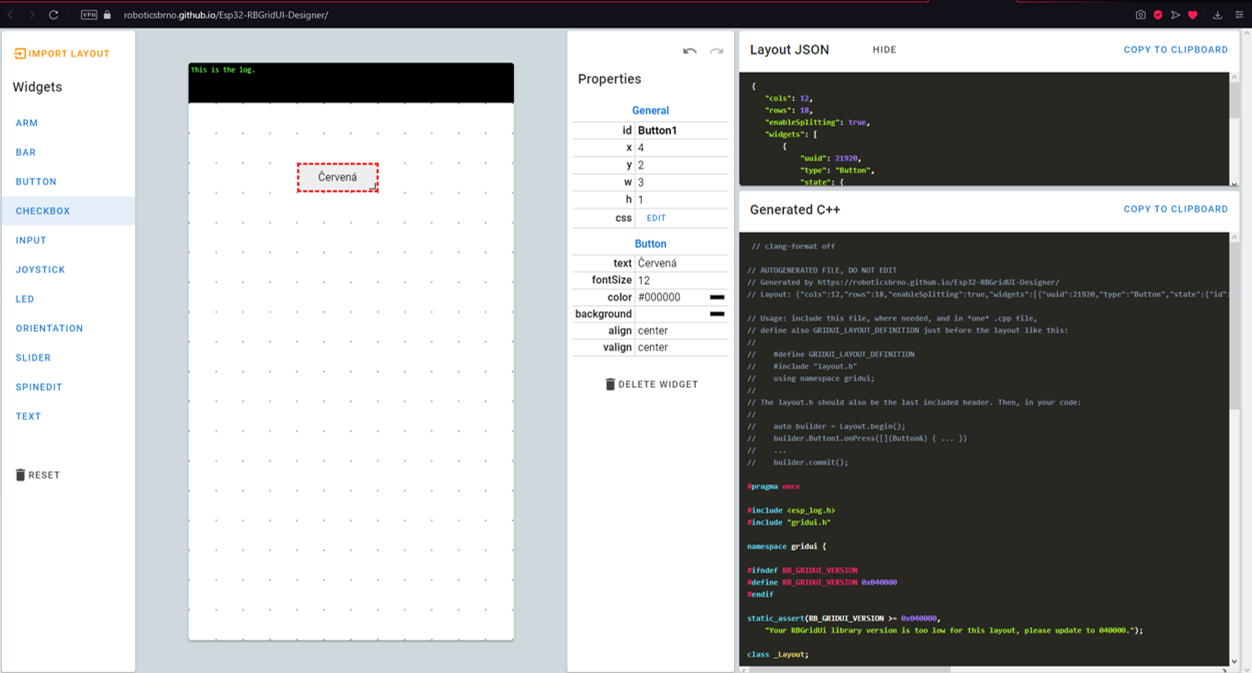
\includegraphics[width=1\textwidth]{img/Esp32-RBGridUI-Designer.png}
	\caption{Prostředí stránky {\em Esp32-RBGridUI-Designer}}
	%	\label{fig:install-sdk-3}
\end{figure}

\begin{enumerate}
	\item Postraní lišta, při kliknutí na jakoukoliv komponentu, je uživatel schopen danou kamponentu přetáhnout na manipulační plochu. 
	\item Manipulační plocha, na kterou se umisťují komponenty z postranní lišty. Nastavuje se tu jejich poloha a umístění. Manipulační plocha určuje vzhled řídící plochy v aplikaci v mobilním telefonu při napojení na daný Wifi modul. 
	\item  Tuto tabulku pro práci s ESP32-DevKitC potřebovat nebudeme.
	\item  Soubor Layout, který je potřeba stáhnout a nahrát do stejné složky jako máme hlavní program. Tento soubor nese informace toho, jakým způsobem jsme nanesli komponenty na manipulační plochu.
	\item Bližší specifikace, určující umístění, barvu, a název tlačítka, které bylo vytvořeno na~manipulační ploše. Tyto informace je možné zde i předělávat a upravovat.
	\item Tlačítko Reset které vymaže veškeré komponenty z Manipulační plochy a tím pádem i z Layoutu.
\end{enumerate}


% {\em Esp32-RBGridUI-Designer} je propojený s aplikací {\em RBControler,} \cite{RBControler}

\section{Vytvoření tlačítek - Jak se používá}
Plán byl vtvořit 4 různá tlačítka, která by přepínala mezi čtyřmi různě barevnými módy světla. Tyto tlačítka byla umístěna na ovládací plochu a přehledně pojmenována. 

Po vytvoření tlačítek v aplikaci, bylo důležité uložit text, který se nacházel v kolonce Layout JSON. Stačilo daný text zkopírovat a vložit do textového souboru layout.txt a příponu .txt přepsat na příponu .hpp. Pak bylo potřeba uchovat tento soubor pro budoucí užití.
\newpage




\chapter{Program a jeho realizace}
Nejefektivnější se mi zdálo psát program v programovacím prostředí \textit{Visual Studio Code}\cite{Visualstudio}, se kterým jsem měla nejvíc zkušeností. 

Jedná se o bezplatný editor zdrojového kódu, vhodný pro programování v jakémkoliv programovacím jazyce, bez potřeby přepínání mezi editory. \textit{Visual Studio Code} má podporu programovacích jazyků jako jsou: Python, Java, C++, Javascript a mnoho dalších. 

Kromě \textit{Visual Studio Code} bylo při realizaci použito i jeho plug-in rozšíření s názvem \textit{PlatformIO}\cite{platformio}, což je soubor knihoven, kompatibilních s knihovnami od \textit{Robotárny}. \textit{Robotárna} toto rozšíření využívá a programuje v něm už léta.  Je skvěle kompatibilní s knihovnami \textit{Arduina} a~knihovnami \textit{SmartLeds}, které byly použity z důvodu jejich jednoduchosti a intuitivnosti při programování s RGB.
%Bylo použito vs. Požila jsem????



\section{Diagram programu }

\begin{figure}[htbp]
	\centering
	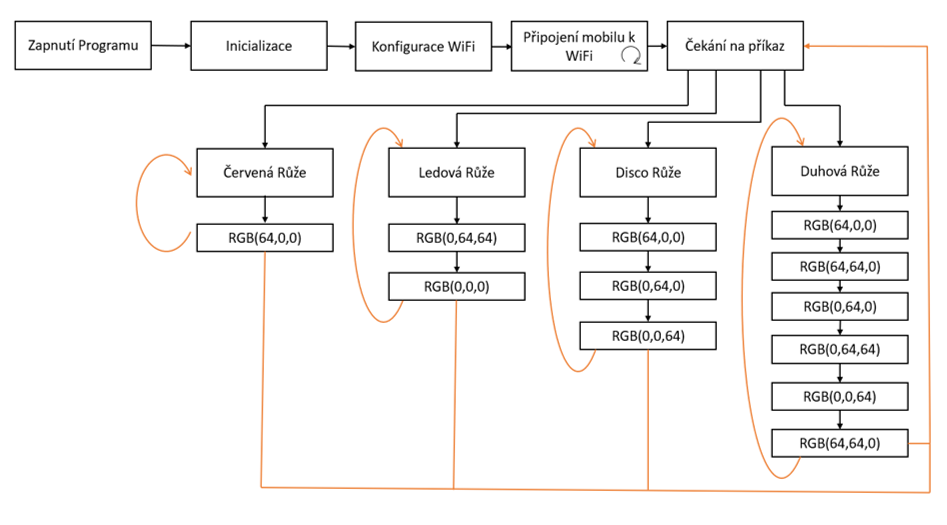
\includegraphics[width=1\textwidth]{img/04 prog/Diagram programu.png}
	\caption{Diagram programu}
	%	\label{fig:install-sdk-3}
\end{figure}

Tento vývojový diagram ukazuje příkazy programu, jak jsou od spuštění (zmáčknutím tlačítka se začne provádět inicializace) až do vypnutí (proces vypnutí může být zahájen v~jakékoliv části programu, stačí jen sepnout tlačítko, a tím přerušit dodávku el energie). 
\newpage

Zde jsou více rozepsané některé části programu:


\subsection{Inicializace}
V této části programu se začnou načítat a spouštět veškeré knihovny zahrnuté v programu. Mezi nimi je i soubor \textit{layout.hpp}, který byl vytvořen a uložen v předchozí kapitole. Jsou zde také informace, který je řídící pin LED pásku a kolik LED bude pásek obsahovat.


\subsection{Konfigurace WiFi a Pipojení k mobilu k Wifi}
%konfigurace = nastavení
V těchto částech programu se kompletně nastaví a zapne vysílaný WiFi signál. Nastaví se jméno a heslo, pod kterými se na WiFi lze připojit. V našem případě se jedná o WiFi s~názvem LEDLED a heslem „ledkyledky“. Dále se nastaví vlastník zařízení, název zařízení, čas kompilace zařízení a za pomoci souboru \textit{layout.hpp} sa nastaví podoba ovládacího panelu v mobilním telefonu. 

Po připojení mobilního telefonu na WiFi a zobrazení ovládacího panelu v aplikaci \textit{RBController} už program v \textit{ESP32-DevKitC} jenom čeká na jeden z naprogramovaných příkazů, aby ho mohl provést.
%Inicializace zařízení? 


\subsection{Příkazy}
Příkazy se v tomhle případě rozumí naše 4 nadefinovaná tlačítka, které jsme si vytvořili v předchozí kapitole. Každé z těchto tlačítek má v programu přidělenou vlastní funkci, kterou po zmáčknutí provede.

Barva světel je naprogramovaná pomocí RGB spektra. V některých případech se jedná o jednu prostou barvu, v jiných o donekonečna se opakující se různobarevný cyklus. 

Tlačítka a jejich příkazy: 
\begin{itemize}
	\item \textbf{Červená růže} – barva LED se nastaví na RGB(64,0,0) – tedy červenou barvu. Touto barvou zařízení září po celou dobu. 
	
	\item \textbf{Ledová růže} – jedná se o cyklický barevný přechod. Světle modré světlo se pomalu rozsvěcuje a poté zhasíná, čímž vytváří pulzující dojem magického předmětu. 
	
	\item \textbf{Disko růže} – cyklus, ve kterém se zběsile střídají 3 barvy (červená, modrá a zelená). Bylo původně spíše myšleno jako recese a nachází se zde pro zastoupení různorodosti barevných kombinací. 
	
	\item \textbf{Duhová růže} – mnohobarevný cyklus, který projde celým barevným spektrem. 
\end{itemize}


Veškeré příkazy jsou provedeny pomocí nadefinované funkce \textit{SetLedAll}, která při zadání 3 čísel automaticky veškeré LED na pásku nastaví na danou RGB barvu, a není potřeba každou jednotlivou LED nastavovat samostatně. Tento příkaz také obsahuje také pár příkazů na stabilizaci LED.

Při programovaní LED pásku nebyla použita maximální intenzita LED pásku. Rozsah RGB je sice od 0 do 255, ale při použití plné intenzity 255 bylo světlo z LED až moc jasné a po delší práci a koukání se na barvy z něj začaly bolet oči a hlava. Proto byla světelná intenzita LED pásku snížena na čtvrtinu. 
\newpage

\chapter{Výroba růže}
Původním záměrem bylo vytvořit svíticí lampičku ve tvaru růže. Vzorem pro výrobu růže byl plastový vršek od lahvičky s uzávěr, s rozměry: přibližně 6~cm široká a 3~cm vysoká. Tato růže byla použita na výrobu formy. Forma byla později opakovaně použita na výrobu tří téměř identických odlitků.
%Mohla jsem se domluvit s umělcem, aby růže byla ze skla, mohla jsem ji vytisknout na 3D tiskárně. Já jsem se ji ale rozhodla odlít, protože mě zaujala práce s křišťálovou pryskyřicí. 

%*Obrázek k vzoru*


\section{Silikonová forma}

Rozhodla jsem se že formu vyrobím z odlévacího silikonu. Odlévací silikony mají skvělé kopírovací vlastnosti a mají i dostatečnou pružnost, potřebnou k dobrému odformování komplikovaných výrobků. Pokud je forma dobře udělaná, lze ji používat opakovaně.



\begin{figure}[htbp]
	\centering
	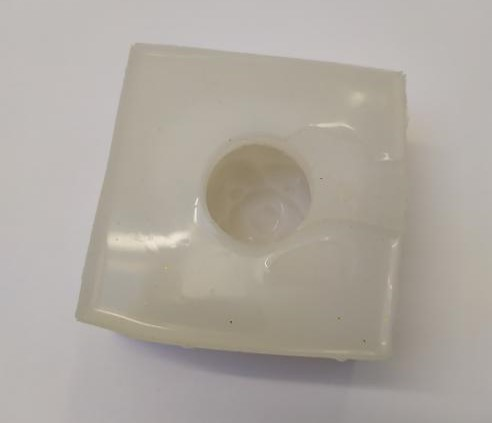
\includegraphics[width=0.5
	\textwidth]{img/05 odl/Silicone mold.jpg}
	\caption{Silikonová forma}
	%	\label{fig:install-sdk-3}
\end{figure}
 

%\subsection{Leukopren žlutý silikon}

\subsection{Adiční silikon GMS A30 (Silikon)}

%Druhým druhem silikonu byl Adiční silikon GMS A30.
Na výrobu formy jsem použila \textit{Adiční silikon GMS A30}\cite{silikon} z internetového obchodu \textit{Levnetmely.cz}\cite{tmely}. Jedná se o dvousložkový, dobře tekutý silikon s velmi dobrou kopírovací schopností, schopný zkopírovat jak povrch obyčejného papíru, tak dřeva s letokruhy.

Tento silikon se používá na výrobu forem, například pro odlévání epoxidové pryskyřice, sádry nebo vosku. Dále se využívá na výrobu těsnění nebo zalévání součástek v elektroprůmyslu.


\subsection{Práce se silikonem}
Balení \textit{Adičního silikonu GMS A30} se skládá ze dvou složek: Složky~A a Složky~B. Tyto dvě složky se musí smíchat v hmotnostním poměru 1:1. Při míchání je potřeba dát pozor, aby se do silikonu nedostaly bublinky, které by mohly znehodnotit formu a zdeformovat kopírovaný tvar.

V případě použití kompresoru by stačilo veškerý vzduch odsát, a tím způsobem se zbavit bublinek. Protože ale kompresor nevlastním nevlastní, malému množství bublinek jsem se nevyhnula. Při práci se silikonem je potřeba dbát na bezpečnost práce a při manipulaci se silikonem mít na sobě ochranné brýle a rukavice.

%*Obrázek formy*

Po přibližně 24 hodinách bývá výsledkem středně tvrdá, odolná silikonová pryžová forma, se skvělým odformováním. V našem případě ale odformování problematizoval komplikovaný tvar květiny.


\begin{figure}[htbp]
	\centering
	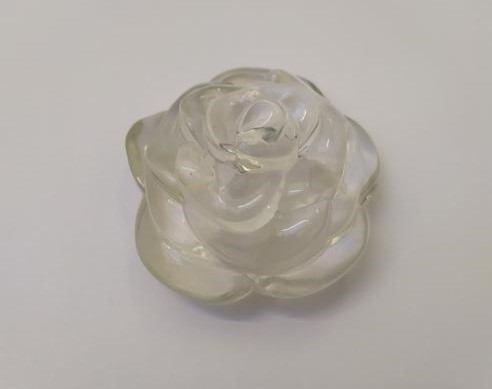
\includegraphics[width=0.5
	\textwidth]{img/05 odl/Rose.jpg}
	\caption{Odlitá růže}
	%	\label{fig:install-sdk-3}
\end{figure}

\section{Pryskyřice}
Křišťálová pryskyřice\cite{pryskyrice} (Epoxy Resin) je dvousložková průhledná odlévací směs často používaná na výrobu bižuterie, různých dekorací nebo glazování povrchů. Dobře se s ní pracuje, její zápach je nízký, a po vytvrdnutí je její povrch lesklý a nesmršťuje se. 

Pro realizaci tohoto projektu byla pryskyřice vybrána z důvodu dobré imitace skla a~zároveň nízké křehkosti tohoto materiálu. 
%Tato pryskyřice byla vybrána i z důvodu, že dobře imituje sklo, ale zase postrádá jeho křehkost.
Při odlévání růže byla konkrétně použita křišťálová pryskyřice od firmy \textit{Pebeo}\cite{pebeo}, sehnatelná v jakémkoliv specializovaném uměleckém obchodě nebo obchodě pro kutily. 


\subsection{Práce s pryskyřicí}

Pro použití pryskyřice je třeba smíchat složku A a složku B. Tyto dvě složky smíchají v~hmotnostním poměru 2:1. Při odvažování je důležitá přesnost. Dále je duležité obě složky dobře promíchat, jinak by mohlo dojít ke špatnému vytvrzení výrobku. Při míchání je třeba dávat pozor, aby se do pryskyřice nedostali bublinky. Poté se daná směs vylije do předem připravené formy nebo na povrch, který chceme glazovat. Pryskyřici trvá 24 až 48 hodin zatvrdne. Opět, křišťálová pryskyřice je chemikálie a proto se, z důvodů možných alergických reakcí a podráždění dýchacích cest, doporučuje při manipulaci s pryskyřicí nosit ochranné brýle, rukavice a respirátor. 

Před vylitím pryskyřice do předem připravené formy je prý vhodné danou formu vytřít speciální vazelínou, která prodlužuje životnost formy a která brání jejímu poškození při vyjímáním odlitku. Tento způsob se ale v našem případě, při odlévání pryskyřičné růže, neosvědčil. Vazelína se smíchala s odlévací pryskyřicí a ve výrobku se vytvořil bílý mléčný kal, který znehodnotil výrobek a pokazil sklovitý dojem pryskyřice.









\input{CHAPTERS/06 - KRABIČKA.tex}

\chapter{Závěr}
Cílem mé dlouhodobé maturitní práce bylo

Nejdříve jsem sestavila obvod, který řídila deska ESP32-DevkitC. Tento obvod se zapínal a vypínal jediným přepínačem, který přesušoval a spojoval obvod. Součástí obvodu je Kromě li-ion baterií a regulátor napětí, které napětí baterií sráží na požadovanou hodnotu. Dodatečně jsem k bateriím vytvořila ještě nabíječku, kterou se kdykoliv baterie mohly znovu nabít. 

Navrhla jsem si v aplikaci ovládací panel a tlačítky a naprogramovala ESP32-DevkitC tak, aby se pomocí jeho WiFi modulu daly jednotlivé módy světla z mobilního zařízení bezdrátově ovládat.  

Dále jsem si vytvořila silikonovou formu, do které jsem opakovaně odlila z křišťálové pryskyřice 3 růže, abych je mohla později použít jako žárovky na jednotlivé prototypy. 

Jako poslední jsem navrhla Základnu, do které se vložil Elektrický obvod, k vrchnímu dílu se připojila růže, která sloužila jako lampička a skrz kterou LED pásek prosvěcoval do prostoru.






%Prototyp světla je ke dni odevzdání ročníkové práce plně funkční. Do budoucna by se dal zkonstruovat obal, ve kterém by byla uložená elektronika (hlavně ESP32-DevKitC) a průhledný tvar, skrz který by LED zářily. Dále by se dalo vyrobit a zprovoznit těchto světel víc a zařídit, aby každé z nich bylo propojeno přes wifi s mobilním telefonem.


%Tato ročníková práce mi dala hodně zabrat. Ne proto, že bych měla složité téma a nebo program by byl složitý na naprogramování, ale problém byl v tom, že jsem se musela často učit pracovat s programy a věcmi, se kterými jsem předtím nepracovala. Naučila jsem se pracovat s ESP32 a inteligentními LED světly, naučila jsem se je programovat a dokonce se napojit na ESP32-DevkitC mobilním telefonem a pomocí něj ESP32-DevkitC ovládat.
%Celkově mě ale práce na této ročníkové práci bavila a dala mi do budoucna spoustu zkušeností, které se jistě budou hodit. 

 



\clearpage
\phantomsection

%\appendix
%\addcontentsline{toc}{chapter}{Přílohy}

% Prilohy
%\chapter{Seznam již vydaných videí} \label{released-videos}
Tato příloha obsahuje kompletní seznam videí vzniklých v~rámci projektu P3D vč. odkazů rozdělených dle jednotlivých témat. \newline
\noindent\It{Pozn.: při kliknutí na odkaz budete přesměrování na stránku korespondujícího videa (pouze v~digitální verzi)}.

\section{Instalace a zprovoznění SolidWorks SDK} \label{videa-instalace}
\href{https://aka.parallaxproduction.cz/instalaceSDK}{Instalace a první spuštění SolidWorks SDK 2020/2021 (aka.parallaxproduction.cz/instSDK)} \newline
\href{https://aka.parallaxproduction.cz/sablony}{Instalace šablon a knihoven norm. dílů ze Sokolské (aka.parallaxproduction.cz/sablony)} \newline
\href{https://aka.parallaxproduction.cz/realview}{Aktivace Realview na necertifikované grafické kartě (aka.parallaxproduction.cz/realview)} \newline

\section{Základy modelování} \label{videa-modelovani}
\href{https://aka.parallaxproduction.cz/jednoducha-pruzina}{Jednoduchá pružina (aka.parallaxproduction.cz/jednoducha-pruzina)} \newline
\href{https://aka.parallaxproduction.cz/j-ozubene-kolo}{Ozubené kolo s~přímým čelním ozubením (aka.parallaxproduction.cz/j-ozubene-kolo)} \newline
\href{https://aka.parallaxproduction.cz/vyk-oz-kolo}{Ozubené kolo pro výkres - obálka (aka.parallaxproduction.cz/vyk-oz-kolo)} \newline
\href{https://aka.parallaxproduction.cz/jednorad-r-kolo}{Jednořadé řetězové kolo (aka.parallaxproduction.cz/jednorad-r-kolo)} \newline
\href{https://aka.parallaxproduction.cz/perodrazka-naboj}{Drážka pro pero v~náboji (aka.parallaxproduction.cz/perodrazka-naboj)} \newline
\href{https://aka.parallaxproduction.cz/perodrazka-hridel}{Drážka pro pero na hřídeli (aka.parallaxproduction.cz/perodrazka-hridel)} \newline

\section{Výkresová dokumentace} \label{videa-vykresy}
\href{https://aka.parallaxproduction.cz/popisove-pole}{Popisové pole a už. vlastnosti na výkrese (aka.parallaxproduction.cz/popisove-pole)} \newline
\href{https://aka.parallaxproduction.cz/vykres-perodrazka-na}{Výkres drážky pro pero v~náboji (aka.parallaxproduction.cz/vykres-perodrazka-hr)} \newline
\href{https://aka.parallaxproduction.cz/vykres-perodrazka-hr}{Výkres drážky pro pero na hřídeli (aka.parallaxproduction.cz/vykres-perodrazka-hr)} \newline

\section{Práce se sestavami} \label{videa-sestavy}
\href{https://aka.parallaxproduction.cz/prejmenovani-dilu}{Přejmenování dílu v~sestavě (aka.parallaxproduction.cz/prejmenovani-dilu)} \newline
\href{https://aka.parallaxproduction.cz/pack-and-go}{Přesun sestavy pomocí Pack and Go... (aka.parallaxproduction.cz/pack-and-go)} \newline

\chapter{Seznam plánovaných témat} \label{planned-videos}
V~následujícím seznamu naleznete další témata, pro která jsou videa plánována.

\subsection*{Nastavení a úpravy SolidWorks}
\begin{itemize}
    \setlength\itemsep{0.05em}
    \item Upgrade SolidWorks na novou verzi (např. 2020 na 2021),
    \item vlastní úpravy uživatelského prostředí,
    \item doplňkové moduly SolidWorks.
\end{itemize}

\subsection*{Základy modelování}
\begin{itemize}
    \setlength\itemsep{0.05em}
    \item Řetěz,
    \item řemen,
    \item plechové díly (série),
    \item svařované konstrukce (série),
    \item další normalizované prvky.
\end{itemize}

\subsection*{Výkresová dokumentace}
\begin{itemize}
    \setlength\itemsep{0.05em}
    \item Kusovník na výkrese sestavy,
    \item 
\end{itemize}

\subsection*{Sestavy}
\begin{itemize}
    \setlength\itemsep{0.05em}
    \item Základní, upřesňující a strojní vazby (série),
    \item konfigurace (pravděpodobně série).
\end{itemize}

%\chapter{Obrazové přílohy}

%\begin{figure}[h]
%    \centering
%    \includegraphics[width=0.85\textwidth]{img/ToBeRemoved/PPSB-T_BOTH.png}
%    \caption{Vizualizace PPSB-T (horní strana vpravo, dolní vlevo).}
%    \label{fig:PPSB-T_VISUAL}
%\end{figure}

\chapter{Vybrané normy}

\begin{table}[] \catcode`\-=12
    \centering
    \begin{tabular}{c|cc|c|c|c|ccccc}
    \multirow{2}{*}{\B{Průměr D}} & \multicolumn{3}{c|}{\B{Rozměr drážky}}      & \multicolumn{2}{c|}{\B{Mezní úchylky hloubky}}                                                                                              & \multicolumn{5}{c}{\B{Rozměry pera}}                                  \\ \cline{2-11} 
                                  & t   & t\subscript{1} & R\subscript{1}       & \multicolumn{1}{l|}{na hřídeli (t)}                                  & \multicolumn{1}{l|}{v náboji (t\subscript{1})}                       & b  & h  & R                     & l\subscript{min} & l\subscript{max} \\ \hline
    6 až 8                        & 1,1 & 0,9            & \multirow{2}{*}{0,2} & \multirow{4}{*}{\begin{tabular}[c]{@{}c@{}}+0,1\\ -0,0\end{tabular}} & \multirow{9}{*}{\begin{tabular}[c]{@{}c@{}}+0,2\\ +0,1\end{tabular}} & 2  & 2  & \multirow{2}{*}{0,25} & 9                & 20               \\
    8 až 10                       & 1,7 & 1,3            &                      &                                                                      &                                                                      & 3  & 3  &                       & 9                & 36               \\ \cline{1-4} \cline{7-11} 
    10 až 12                      & 2,4 & 1,6            & \multirow{4}{*}{0,4} &                                                                      &                                                                      & 4  & 4  & \multirow{4}{*}{0,5}  & 10               & 45               \\
    12 až 17                      & 2,9 & 2,1            &                      &                                                                      &                                                                      & 5  & 5  &                       & 12               & 56               \\ \cline{5-5}
    17 až 22                      & 3,5 & 2,5            &                      & \multirow{8}{*}{\begin{tabular}[c]{@{}c@{}}+0,2\\ -0,0\end{tabular}} &                                                                      & 6  & 6  &                       & 16               & 70               \\
    22 až 30                      & 4,1 & 2,9            &                      &                                                                      &                                                                      & 8  & 7  &                       & 20               & 90               \\ \cline{1-4} \cline{7-11} 
    30 až 38                      & 4,7 & 3,3            & \multirow{6}{*}{0,6} &                                                                      &                                                                      & 10 & 8  & \multirow{6}{*}{0,7}  & 25               & 110              \\
    38 až 44                      & 4,9 & 3,1            &                      &                                                                      &                                                                      & 12 & 8  &                       & 32               & 140              \\
    44 až 50                      & 5,5 & 3,5            &                      &                                                                      &                                                                      & 14 & 9  &                       & 40               & 180              \\ \cline{6-6}
    50 až 58                      & 6,2 & 3,8            &                      &                                                                      & \multirow{3}{*}{\begin{tabular}[c]{@{}c@{}}+0,4\\ +0,2\end{tabular}} & 16 & 10 &                       & 45               & 200              \\
    58 až 65                      & 6,8 & 4,2            &                      &                                                                      &                                                                      & 18 & 11 &                       & 50               & 220              \\
    65 až 75                      & 7,4 & 4,6            &                      &                                                                      &                                                                      & 20 & 12 &                       & 56               & 250             
    \end{tabular}
    \caption{Výběr z~normy ČSN 02 2562 - Pera těsná\cite{ST}}
    \label{tab:pera-tesna}
\end{table}

\begin{figure}[htbp]
    \centering
    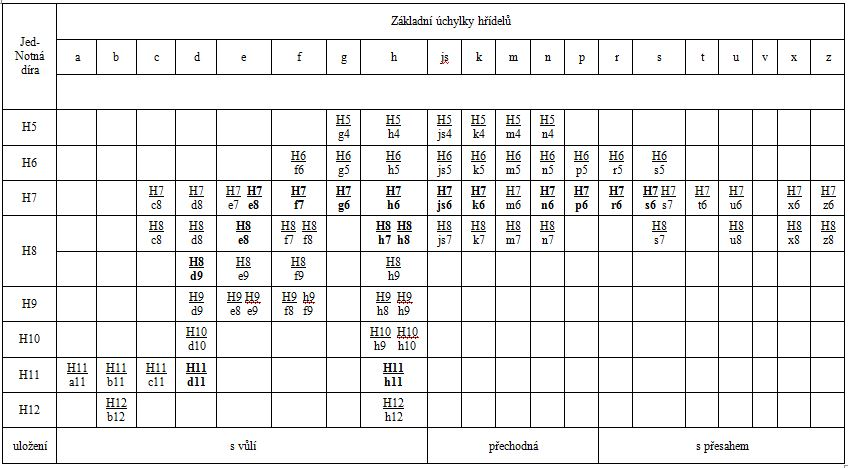
\includegraphics[width=1\textwidth]{img/jednotna-dira.JPG}
    \caption{Soustava jednotné díry, tučně zvýrazněné hodnoty jsou doporučené, převzato z~\cite{ELUC-DIRA}}
    \label{fig:jednotna-dira}
\end{figure}

\begin{figure}[htbp]
    \centering
    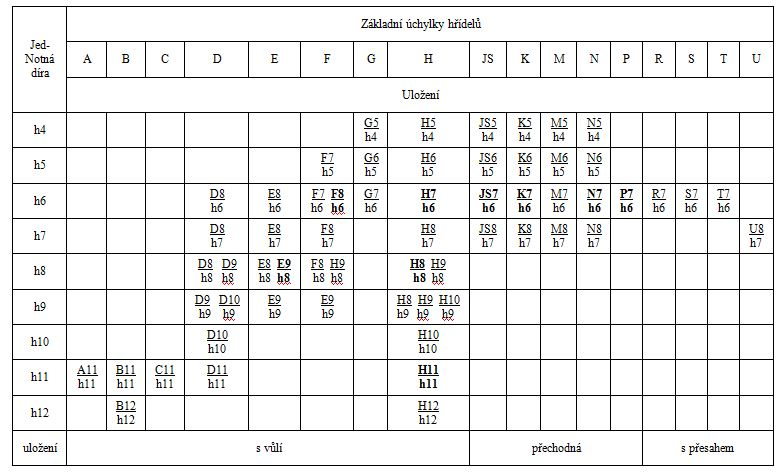
\includegraphics[width=1\textwidth]{img/jednotna-hridel.JPG}
    \caption{Soustava jednotného hřídele, tučně zvýrazněné hodnoty jsou doporučené, převzato z~\cite{ELUC-HRIDEL}}
    \label{fig:jednotna-hridel}
\end{figure}

\input literatura.tex


\listoffigures
\addcontentsline{toc}{chapter}{Seznam obrázků}

%\listoftables
%\addcontentsline{toc}{chapter}{Seznam tabulek}

\end{document}
%todo zadání dodělat 
%todo vlna 
